\epi{"Go has pointers but not pointer arithmetic. You cannot use a pointer
variable to walk through the bytes of a string."}{\textit{Go For C++
Programmers}\\{\textsc{GO AUTHORS}}}
\noindent{}
Go has pointers.
There is however no pointer arithmetic, so they act more like
references than pointers that you may know from C. Pointers 
are useful.
Remember that when you call a function in Go, the variables are
\emph{pass-by-value}. So, for efficiency and the possibility to modify a
passed value \emph{in} functions we have pointers.

You declare a pointer by prefixing the type with an
'\key{*}':
\lstinline{var p *int}. Now \var{p} is a pointer to an integer value.
All newly declared variables are assigned their zero value and pointers
are no difference. A newly declared, or just a pointer that points to
nothing has a \first{nil}{nil}-value. In other languages this is often called
a NULL pointer in Go it is just \var{nil}. To make 
a pointer point to something you can use the \first{address-of operator}{operator!address-of}
(\func{\&}), which we do on line 5:
\begin{lstlisting}[caption=Use of a pointer,label=src:pointers]
var p *int
fmt.Printf("%v", p) |\coderemark{Prints \var{nil}}|

var i int	    |\coderemark{Declare integer variable \var{i}}|
p = &i		    |\coderemark{Make \var{p} point to \var{i}}|

fmt.Printf("%v", p) |\coderemark{Prints something like \var{0x7ff96b81c000a}}|
\end{lstlisting}

More general: \var{*X} is a pointer to an \type{X}; \var{[3]X} is an
array of three \type{X}s. The
types are therefore really easy to read just read out the names of the
type modifiers: \type{[]} declares an array slice;
'\key{*}'
declares a pointer; \type{[size]} declares an array. So
\type{[]*[3]*X} is an array slice of pointers to arrays of three
pointers to \type{X}s (also see figure \ref{fig:pointers}).
\begin{figure}[h]
\caption[Pointers and types]{Pointers and types, the values \var{v} all have type \type{X}}
\label{fig:pointers}
\begin{center}
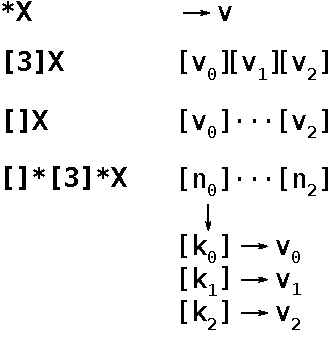
\includegraphics[scale=0.65]{fig/pointers.pdf}
\end{center}
\end{figure}

Dereferencing a pointer is done by prefixing the pointer variable with
'\type{*}':
\begin{lstlisting}[caption=Dereferencing a pointer,label=src:deref]
p = &i			|\coderemark{Take the address of \var{i}}|
*p = 8			|\coderemark{Change the value of \var{i}}|
fmt.Printf("%v\n", *p)  |\coderemark{Prints 8}|
fmt.Printf("%v\n", i)	|\coderemark{Idem}|
\end{lstlisting}

\label{main:pointer arithmetic}
As said, there is no pointer arithmetic, so if you write:
\lstinline{*p++}, it is interpreted as \lstinline{(*p)++}: first
dereference and then increment the value.\index{operator!increment}
\footnote{See exercise \ref{ex:pointer arithmetic}.}

\section{Allocation}
Go also has garbage collection, meaning that you don't have to worry about
memory deallocation. Of course almost every language
since 1980 has this, but it is nice to see garbage collection in a
C-like language.

To allocate memory Go has two primitives, \key{new} and \key{make}. They do different
things and apply to different types, which can be confusing, but the
rules are simple.
The following sections show how to handle allocation
in Go and hopefully clarifies the somewhat artificial distinction between
\first{\key{new}}{built-in!new} and \first{\key{make}}{built-in!make}. 

\subsection{Allocation with new}
\label{sec:allocation with new}
The built-in function \key{new} is 
essentially the same as its namesakes in other languages: \func{new(T)}
allocates zeroed storage for a new item of type \type{T} and returns its
address, a value of type \type{*T}. In Go terminology, it returns a pointer to
a newly allocated zero value of type \type{T}. This is important to
remember:
\begin{lbar}[]
\key{new} returns \emph{pointers}.
\end{lbar}

This
means a user of the data structure can create one with \key{new} and get
right to work. For example, the documentation for \func{bytes.Buffer} states
that "the zero value for Buffer is an empty buffer ready to use."
Similarly, \func{sync.Mutex} does not have an explicit constructor or Init
method. Instead, the zero value for a \func{sync.Mutex} is defined to be an
unlocked mutex.

The zero-value-is-useful property works transitively. Consider this type
declaration. See section "\titleref{sec:defining your own}" on page
\pageref{sec:defining your own}.

\begin{lstlisting}
type SyncedBuffer struct {
    lock    sync.Mutex
    buffer  bytes.Buffer
}
\end{lstlisting}
Values of type \type{SyncedBuffer} are also ready to use immediately upon
allocation or just declaration. In this snippet, both \var{p} and
\var{v} will work
correctly without further arrangement.
\begin{lstlisting}
p := new(SyncedBuffer)  |\coderemark{Type *SyncedBuffer}|
var v SyncedBuffer      |\coderemark{Type  SyncedBuffer}|
\end{lstlisting}

\subsection{Allocation with make}
\label{sec:allocation with make}
Back to allocation. The built-in function \func{make(T, args)} serves a purpose
different from \func{new(T)}. It creates slices, maps, and channels only, and
it returns an initialized (not zero) value of type \type{T}, not
\type{*T}. The reason
for the distinction is that these three types are, under the covers,
references to data structures that must be initialized before use. A
slice, for example, is a three-item descriptor containing a pointer to
the data (inside an array), the length, and the capacity; until those
items are initialized, the slice is \type{nil}. For slices, maps, and channels,
\key{make} initializes the internal data structure and prepares the value for
use. 

\begin{lbar}[]
\key{make} returns initialized (non zero) \emph{values}.
\end{lbar}

For instance,
\lstinline{make([]int, 10, 100)}
allocates an array of 100 ints and then creates a slice structure with
length 10 and a capacity of 100 pointing at the first 10 elements of the
array. In contrast,
\lstinline{new([]int)} returns
a pointer to a newly allocated, zeroed slice structure, that is, a
pointer to a \type{nil} slice value.

These examples illustrate the difference between \key{new} and
\key{make}.
\begin{lstlisting}
var p *[]int = new([]int)       // allocates slice structure; *p == nil
				// rarely useful
var v  []int = make([]int, 100) // v refers to a new array of 100 ints

// Unnecessarily complex:
var p *[]int = new([]int)
*p = make([]int, 100, 100)

// Idiomatic:
v := make([]int, 100)
\end{lstlisting}
Remember that \key{make} applies only to maps, slices and channels and does
not return a pointer. To obtain an explicit pointer allocate with
\key{new}.

\begin{lbar}[\lstinline{new} allocates; \lstinline{make} initializes]
The above two paragraphs can be summarized as:\\
\lstinline{new(T)} returns \var{*T} pointing to a zeroed \var{T}\\
\lstinline{make(T)} returns an initialized \var{T}\\
And of course \lstinline{make} is only used for slices, maps and channels.
\end{lbar}

\subsection{Constructors and composite literals}
\label{sec:constructors and composite literals}
Sometimes the zero value isn't good enough and an initializing
constructor is necessary, as in this example taken from the package
\package{os}.
\begin{lstlisting}
func NewFile(fd int, name string) *File {
    if fd < 0 {
        return nil
    }
    f := new(File)
    f.fd = fd
    f.name = name
    f.dirinfo = nil
    f.nepipe = 0
    return f
}
\end{lstlisting}
There's a lot of boiler plate in there. We can simplify it using a
\first{composite literal}{literal!composite}, which is an expression that 
creates a new instance each time it is evaluated.

\begin{lstlisting}
func NewFile(fd int, name string) *File {
    if fd < 0 {
        return nil
    }
    f := File{fd, name, nil, 0}	|\coderemark{Create a new \type{File}}|
    return &f			|\coderemark{Return the address of \var{f}}|
}
\end{lstlisting}
It is OK to return the address of a local variable;
the storage associated with the variable survives after the function
returns.

In fact, taking the address of a composite literal allocates a
fresh instance each time it is evaluated, so we can combine these last
two lines.\footnote{Taking the address of a composite literal tells the 
compiler to allocate it on the heap, not the stack.}
\begin{lstlisting}
return &File{fd, name, nil, 0}
\end{lstlisting}
The items (called \first{fields}{fields} of a composite 
literal are laid out in order and must all be
present. However, by labeling the elements explicitly as field:value
pairs, the initializers can appear in any order, with the missing ones
left as their respective zero values. Thus we could say

\begin{lstlisting}
return &File{fd: fd, name: name}
\end{lstlisting}
As a limiting case, if a composite literal contains no fields at all, it
creates a zero value for the type. The expressions
\lstinline{new(File)} and 
\lstinline|&File{}| are equivalent.

Composite literals can also be created for arrays, slices, and maps,
with the field labels being indices or map keys as appropriate. In these
examples, the initializations work regardless of the values of
\var{Enone},
\var{Eio}, and \var{Einval}, as long as they are distinct.
\begin{lstlisting}
ar := [...]string   {Enone: "no error", Eio: "Eio", Einval: "invalid argument"}
sl := []string      {Enone: "no error", Eio: "Eio", Einval: "invalid argument"}
ma := map[int]string{Enone: "no error", Eio: "Eio", Einval: "invalid argument"}
\end{lstlisting}

\section{Defining your own types}
\label{sec:defining your own}
Of course Go allows you to define new types, it does this 
with the \first{\key{type}}{keyword!type} keyword: 
\begin{lstlisting}
type foo int
\end{lstlisting}
Creates
a new type \lstinline{foo} which acts like an \lstinline{int}.
Creating more sophisticated types is done with the
\first{\key{struct}}{keyword!struct}
keyword.
An example would be when we want record somebody's name (\type{string})
and age (\type{int}) in a single structure and make it a new type:
\lstinputlisting[label=src:struct,caption=Structures]{src/struct.go}
Apropos, the output of \lstinline{fmt.Printf("%v\n", a)} is 
\begin{display}
&\{Pete 42\}
\end{display}
That is nice!
Go knows how to print your structure. If you
only want to print one, or a few, fields of the structure you'll
need to use \verb|.<field name>|. For example to only print the name:
\begin{lstlisting}
fmt.Printf("%s", a.name) |\coderemark{\%s formats a string}|
\end{lstlisting}
%% add text if a is a pointer

\subsection{More on structure fields}
As said each item in a structure is called a \index{field}{field}.
A struct with no fields:
\begin{lstlisting}
struct {}
\end{lstlisting}
Or one with five fields:
\begin{lstlisting}
struct {
        x, y int
        _ float64  |\coderemark{Padding}|
        A *[]int
        F func()
}
\end{lstlisting}
If you omit the name for a field, you create an 
\first{anonymous field}{field!anonymous}, for instance:
\begin{lstlisting}
struct {
        T1        |\coderemark{Field name is T1}|
        *T2       |\coderemark{Field name is T2}|
        P.T3      |\coderemark{Field name is T3}|
        x, y int  |\coderemark{Field names are x and y}|
}
\end{lstlisting}
Note the field names that start with a capital letter are exported, i.e. can be
set or read from other packages. Field names that start with a lowercase are private
to the current package. The same goes for functions defined in packages, see chapter
\ref{chap:packages}.

\subsection{Methods}
\label{sec:methods}
If you create functions that works on your newly defined type, you can
take two routes:
\begin{enumerate}
\item Create a function that takes the type as an argument.
\begin{lstlisting}
func doSomething(in1 *NameAge, in2 int) { /* ... */ }
\end{lstlisting}
This is (you might have guessed) a \first{\emph{function call}}{function!call}.
\item Create a function that works on the type (see \emph{receiver} in
listing \ref{src:function definition}):
\begin{lstlisting}
func (in1 *NameAge) doSomething(in2 int) { /* ... */ }
\end{lstlisting}
This is a \first{\emph{method call}}{method call}, which can be
used as: 
\begin{lstlisting}
var n *NameAge
n.doSomething(2)
\end{lstlisting}
\end{enumerate}
But keep the following in mind, this is quoted from \cite{go_spec}:
\begin{quote}
If \type{x} is
addressable and \lstinline{&x}'s method set contains \func{m}, 
\lstinline{x.m()} is shorthand for \lstinline{(&x).m()}.
\end{quote}
In the above case this means that the following is \emph{not} an 
error:
\begin{lstlisting}
var n NameAge	    |\coderemark{Not a pointer}|
n.doSomething(2)    
\end{lstlisting}
Here Go will search the method list for \var{n} of type \type{NameAge},
come up empty and will then \emph{also} search the method list for
the type \type{*NameAge} and will translate this call to
\lstinline{(&n).doSomething(2)}.
Whether to use a function or method is entirely up to the programmer, but
if you want to satisfy an interface (see the next chapter) you must use
methods.

There is a subtle but major difference between the following type
declarations. Also see \cite[section~"Type Declarations"]{go_spec}.
Suppose we have:
\begin{lstlisting}
// A Mutex is a data type with two methods, Lock and Unlock.
type Mutex struct         { /* Mutex fields */ }
func (m *Mutex) Lock()    { /* Lock implementation */ }
func (m *Mutex) Unlock()  { /* Unlock implementation */ }
\end{lstlisting}
We now create two type in two different manors:
\begin{itemize}
\item \lstinline|type NewMutex Mutex|;
\item \lstinline|type PrintableMutex struct { Mutex }|.
\end{itemize}
Now \var{NewMutux} has the same memory layout as \var{Mutex}, but
is doesn't have any of the methods of \var{Mutex}. In other words
its method set is empty.
But \var{PrintableMutex} \emph{has} \first{\emph{inherited}}{methods!inherited} the 
method set from \var{Mutex}.
In the words of \cite{go_spec}:
\begin{quote}
The method set of \var{*PrintableMutex} contains the methods
\func{Lock} and \func{Unlock} bound to its anonymous field \var{Mutex}.
\end{quote}

\section{Conversions}
\label{sec:conversions}
Sometimes you want to convert a type to another type. 
This is possible in Go, but
there are some rules. For starters, converting from one value to another
is done by functions and not all conversions are allowed.

\begin{table}[H]
\begin{center}
\caption[Valid conversions]{Valid conversions, 
\lstinline{float64} works the same as \lstinline{float32}}
\label{tab:convesion}
\begin{tabular}{llllllll}
    \textbf{From}	 &  \verb|xb []byte|& \verb|xi []int| & \verb|xr []rune| & \verb|s string|     & \verb|f float32|	&  \verb|i int|	\\ \cmidrule(r){1-7}
      \textbf{To}	 &		    &                 &   &			   &			& \\ \cmidrule(r){1-1}
  \verb|[]byte|    & $\texttimes$	    &                 &   & \verb|[]byte(s)|	   &			& \\
  \verb|[]int|     &		    & $\texttimes$            &   & \verb|[]int(s)|	   &			& \\
  \verb|[]rune|    &                &                         & $\texttimes$  &  \verb|[]rune(s)| &                    & \\
  \verb|string|    &\verb|string(xb)| &\verb|string(xi)|      &  \verb|string(xr)| &	$\texttimes$	   &			& \\
 \verb|float32|	 &		    &                         &   &			   & $\texttimes$	& \verb|float32(i)|\\
     \verb|int|	 &		    &                         &   &			   & \verb|int(f)|	& $\texttimes$ \\
%%\bottomrule
\end{tabular}

\end{center}
\end{table}

\begin{itemize}
\item{
From a \lstinline{string} to a slice of bytes or ints.
\begin{lstlisting}
mystring := "hello this is string"
\end{lstlisting}

\begin{lstlisting}
byteslice := []byte(mystring)
\end{lstlisting}
Converts to a \type{byte} slice, each \type{byte} contains the integer value
of the corresponding byte in the string. Note that as strings in Go
are encoded in UTF-8 some characters in the string may end up in 1, 2, 3
or 4 bytes.
\begin{lstlisting}
intslice  := []int(mystring)
\end{lstlisting}
Converts to an \type{int} slice, each \type{int} contains a Unicode code
point. Every character from the string is corresponds to one integer.
}
\item{
From a slice of bytes or ints to a \lstinline{string}.
\begin{lstlisting}
b := []byte{'h','e','l','l','o'} |\coderemark{Composite literal}|
s := string(b)
i := []int{257,1024,65} 
r := string(i)
\end{lstlisting}
}
\end{itemize}
For numeric values the following conversion are defined:
\begin{itemize}
\item{Convert to a integer with a specific (bit) length: 
\lstinline{uint8(int)};}
\item{From floating point to an integer value: 
\lstinline{int(float32)}. This discards the fraction part
from the floating point value;}
\item{The other way around: \lstinline{float32(int)};}
\end{itemize}

\subsection{User defined types and conversions}
How can you convert between the types you have defined
yourself?
We create two types here \type{Foo} and \type{Bar}, where
\lstinline{Bar} is an alias for \type{Foo}:
\begin{lstlisting}
type foo struct { int }  |\coderemark{Anonymous struct field}|
type bar foo             |\coderemark{bar is an alias for foo}|
\end{lstlisting}

Then we:
\begin{lstlisting}
var b bar = bar{1} |\coderemark{Declare \var{b} to be a \type{bar}}|
var f foo = b	   |\coderemark{Assign \var{b} to \var{f}}|
\end{lstlisting}
Which fails on the last line with:

\noindent\error{cannot use b (type bar) as type foo in assignment}

\noindent{}This can be fixed with a conversion:
\begin{lstlisting}
var f foo = foo(b)
\end{lstlisting}
Note the converting structures that are not identical in their fields
is more difficult. Also note that converting \lstinline{b} to a plain
\type{int} also fails; an integer is not the same as a structure containing
an integer.

\section{Exercises}
\begin{Exercise}[title={Pointer arithmetic},difficulty=1]
\label{ex:pointer arithmetic}
\Question
In the main text on page \pageref{main:pointer arithmetic}
there is the following text:

\begin{quote}
\ldots there is no pointer arithmetic, so if you write:
\lstinline{*p++}, it is interpreted as \lstinline{(*p)++}: first
dereference and then increment the value.
\end{quote}
When you increment a value like this, for which types will it work?
\Question Why doesn't it work for all types?

\end{Exercise}

\begin{Answer}
\Question This will only work for pointers to point to numerical (\type{int, uint}, etc) values.
\Question The \func{++} is only defined for numerical types and because there
is no operator overloading in Go it fails (compilation error) otherwise.
\end{Answer}


\begin{Exercise}[title={使用 interface 的 map 函数},difficulty=6]
\label{ex:map function interfaces}
\Question
使用练习 Q\ref{ex:map function} 的答案,利用 interface 使其更加通用。
\end{Exercise}

\begin{Answer}
\Question
\lstinputlisting[label=src:map,caption=Go 中更加通用的 map 函数]{ex-beyond/src/map.go}
\end{Answer}




\begin{Exercise}[title={指针},difficulty=6]
\label{ex:pointers}

\Question
假设定义了下面的结构:
\begin{lstlisting}
type Person struct {
    name string
    age	 int
}
\end{lstlisting}

下面两行之间的区别是什么?
\begin{lstlisting}
var p1 Person
p2 := new(Person)
\end{lstlisting}

\Question
下面两个内存分配的区别是什么?
\begin{lstlisting}[numbers=none]
func Set(t *T) {
    x = t
}
\end{lstlisting}
和
\begin{lstlisting}[numbers=none]
func Set(t T) {
    x= &t
}
\end{lstlisting}
\end{Exercise}

\begin{Answer}
\Question
第一行:\lstinline{var p1 Person} 分配了
\texttt{Person}-\emph{值} 给 \var{p1}。\var{p1} 的类型是
\type{Person}。

第二行:\lstinline{p2 := new(Person)} 分配了内存并且将\emph{指针}赋值给
\var{p2}。\var{p2} 的类型是 \type{*Person}。

\Question
在第二个函数中,\var{x} 指向一个新的(堆上分配的)变量
\var{t},其包含了实际参数值的副本。

在第一个函数中,\var{x} 指向了 \var{t} 指向的内容,
也就是实际上的参数指向的内容。

因此在第二个函数,我们有了``额外''的变量存储了相关值的副本。
\end{Answer}


\begin{Exercise}[title={Linked List},difficulty=1]
\label{ex:linkedlist}
\Question
\label{ex:linkedlist q1}
Make use of the package \package{container/list} to create
a (double) linked list. Push the values 1, 2 and 4 to the list and then
print it.

\Question
Create your own linked list implementation. And perform the same actions
as in question \ref{ex:linkedlist q1}
\end{Exercise}

\begin{Answer}
\Question

\Question
\end{Answer}


\begin{Exercise}[title={Cat},difficulty=1]
\label{ex:cat}
\Question \label{ex:cat q1} 编写一个程序,模仿 Unix 的 \prog{cat} 程序。
对于不知道这个程序的人来说,下面的调用显示了文件 \dir{blah} 的内容:
\begin{display}
\pr cat blah
\end{display}

\Question 使其支持 \-n 开关,用于输出每行的行号。

\Question 上面问题中,\ref{q:cat} 提供的解决方案存在一个~Bug。
你能定位并修复它吗?
\end{Exercise}

\begin{Answer}
\Question 下面是 \prog{cat} 的实现,同样支持 \-n 输出每行的行号。
\label{q:cat}
\lstinputlisting[label=src:cat,caption=cat 程序]{ex-beyond/src/cat.go}
\showremarks

\Question 当最后一行不包括换行符时,这个~Bug 就会出现。
更糟糕的情况是,当输入只有一行且没有换行符的时候,什么也不显示。
下面的程序是一个更好的解决方案。
\lstinputlisting[label=src:cat2,caption=一个更好的~cat 程序]{ex-beyond/src/cat2.go}
\end{Answer}


\begin{Exercise}[title={方法调用},difficulty=2]
\label{ex:methodcalls}
\Question \label{ex:methodcalls q1} 假设有下面的程序。
要注意的是包 \package{container/vector} 曾经是 Go 的一部分,但是当内建的
\func{append} 出现后,就被移除了。
然而,对于当前的问题这不重要。这个包实现了有 push 和 pop 方法的栈结构。

\begin{lstlisting}
package main

import "container/vector"

func main() {
	k1 := vector.IntVector{}
	k2 := &vector.IntVector{}
	k3 := new(vector.IntVector)
	k1.Push(2)
	k2.Push(3)
	k3.Push(4)
}
\end{lstlisting}
\var{k1},\var{k2} 和 \var{k3} 的类型是什么?

\Question 当前,这个程序可以编译并且运行良好。在不同类型的变量上 \func{Push}
都可以工作。\func{Push} 的文档这样描述:
\begin{quote}
func (p *IntVector) Push(x int)
Push 增加 x 到向量的末尾。
\end{quote}
那么接受者应当是 \type{*IntVector} 类型,为什么上面的代码(Push 语句)可以正确工作?
above (the Push statements) work correct then?

\end{Exercise}

\begin{Answer}
\Question \var{k1} 的类型是 \type{vector.IntVector}。为什么?
这里使用了符号 \verb|{}|,因此获得了类型的值。
变量 \var{k2} 是 \type{*vector.IntVector},因为获得了复合语句的地址(\verb|&|)。
而最后的 \var{k3} 同样是 \type{*vector.IntVector} 类型,因为 \func{new}
返回该类型的指针。

\Question 在 \cite{go_spec} 的``调用''章节,有这样的描述:
\begin{quote}
当 \var{x} 的方法集合包含 \func{m},
并且参数列表可以赋值给 \func{m} 的参数,方法调用 \func{x.m()} 是合法的。
如果 \var{x} 可以被地址化,而 \var{\&x} 的方法集合包含 \func{m},
\func{x.m()} 可以作为 \func{(\&x).m()} 的省略写法。
\end{quote}
换句话说,由于 \var{k1} 可以被地址化,而 \type{*vector.IntVector}
\emph{具有} \func{Push} 方法,调用 \lstinline{k1.Push(2)} 被 Go 转换为 
\lstinline{(&k1).Push(2)} 来使型系统愉悦(也使你愉悦——现在你已经了解到这一点)。
\footnote{参阅本章的第 ``\titleref{sec:methods}'' 节。}

\end{Answer}


\cleardoublepage
\section{Answers}
\shipoutAnswer
